
%% conf_paper.tex

\documentclass[conference]{IEEEtran}
% Add the compsoc option for Computer Society conferences.
%
% If IEEEtran.cls has not been installed into the LaTeX system files,
% manually specify the path to it like:
% \documentclass[conference]{../sty/IEEEtran}


% *** GRAPHICS RELATED PACKAGES ***
%
\ifCLASSINFOpdf
   \usepackage[pdftex]{graphicx}
  % declare the path(s) where your graphic files are
   \graphicspath{{../pdf/}{../jpeg/}}
  % and their extensions so you won't have to specify these with
  % every instance of \includegraphics
   \DeclareGraphicsExtensions{.pdf,.jpeg,.png}
\else
  % or other class option (dvipsone, dvipdf, if not using dvips). graphicx
  % will default to the driver specified in the system graphics.cfg if no
  % driver is specified.
   \usepackage[dvips]{graphicx}
  % declare the path(s) where your graphic files are
   \graphicspath{{../eps/}}
  % and their extensions so you won't have to specify these with
  % every instance of \includegraphics
   \DeclareGraphicsExtensions{.eps}
\fi

%=========================================================
% Latex Packages
%=========================================================
\usepackage{listings}
\usepackage{xspace}
\usepackage[colorlinks=true,linkcolor=blue,citecolor=blue,urlcolor=blue]{hyperref}
\usepackage[colorinlistoftodos,textwidth=2.5cm,shadow]{todonotes}

%=========================================================
% Other
%=========================================================

\usepackage{color}
\usepackage{listings}


%\newcommand{\comment}[1]{\textcolor{red}{#1}}
\definecolor{keywordcolor}{rgb}{0.5,0,0.33}
\definecolor{identifiercolor}{rgb}{0,0,0.75}
%\definecolor{commentcolor}{rgb}{0.25,0.5,0.37}
\definecolor{commentcolor}{rgb}{0.3,0.3,0.3} 

\lstdefinelanguage{bon} {
  morekeywords={class_chart,indexing,explanation,part,query,command,constraint,
  end,deferred,effective,persistent,require,ensure,invariant,feature,class,
  static_diagram,component,old,not,inherit,delta,for_all,such_that,it_holds,Current,Lockset,when,monitors_for,max,concurrency,concurrent,guarded,locks,special,failure,sequential,atomic},
  morekeywords={[2]LOCK,SEMAPHORE,BOOLEAN,INTEGER,REAL,SEQUENCE,MAIN,EXCEPTION,NO_SEATS,BARBER_SHOP,CUSTOMER,BARBER},
  morekeywords={[3]},
  morecomment=[l]{--}, morestring=[b]", morestring=[d]'
  }[keywords,comments,strings]

\lstdefinestyle{bon}{language={bon},showstringspaces={false},
  basicstyle={\scriptsize\ttfamily\mdseries},
  keywordstyle={\color{keywordcolor}},
  keywordstyle={[2]\color{black}\bfseries},
  keywordstyle={[3]\color{black}\bfseries},
  identifierstyle={\color{identifiercolor}},
  commentstyle={\color{commentcolor}},
  frame=lines}

\lstdefinestyle{boninline}{language={bon},showstringspaces={false},
  basicstyle={\ttfamily\mdseries},
  keywordstyle={\color{black}},
  keywordstyle={[2]\color{black}\bfseries},
  keywordstyle={[3]\color{black}\bfseries},
  identifierstyle={\color{black}\mdseries},
  commentstyle={\color{black}},
  frame=lines,
  columns=fullflexible,
  breaklines=true}
\lstset{style=bon, columns=fullflexible, keepspaces=true, 
        frame=topline, captionpos=b}

%=========================================================
% Generic Macros
%=========================================================

\newcommand{\lstbon}[1]{\lstinline[style=boninline]{#1}} 
\newcommand{\lstjava}[1]{\lstinline[style=jml2inline]{#1}} 

\newcommand{\eg}{e.g.,\xspace}
\newcommand{\ie}{i.e.,\xspace}
\newcommand{\etc}{etc.\xspace}
\newcommand{\vs}{vs.\xspace}
\newcommand{\etal}{et.~al.\xspace}

% Todos
\newcommand{\note}[1]{\todo[inline,color=red!40]{#1}}

% correct bad hyphenation here
\hyphenation{op-tical net-works semi-conduc-tor}

% =========================================================

\begin{document}
%
% paper title
% can use linebreaks \\ within to get better formatting as desired
\title{A Rigorous Methodology for Analyzing and Designing Plug-ins}


% author names and affiliations
% use a multiple column layout for up to three different
% affiliations
\author{
\IEEEauthorblockN{ Marieta V. Fasie}
\IEEEauthorblockA{DTU Compute\\Technical University of Denmark\\
DK-2800 Lyngby, Denmark\\
Email: marietafasie@gmail.com}

\and

\IEEEauthorblockN{ Anne E. Haxthausen}
\IEEEauthorblockA{DTU Compute\\Technical University of Denmark\\
DK-2800 Lyngby, Denmark\\
Email: ah@imm.dtu.dk}

\and

\IEEEauthorblockN{Joseph Kiniry}
\IEEEauthorblockA{DTU Compute\\Technical University of Denmark\\
DK-2800 Lyngby, Denmark\\
Email: jkin@imm.dtu.dk}}

% use for special paper notices
%\IEEEspecialpapernotice{(Invited Paper)}


% make the title area
\maketitle

% =========================================================
% Abstract
% =========================================================

\begin{abstract}
%\boldmath
  Today, GUI plug-ins development is typically done in a very ad-hoc
  way, where developers dive directly into implementation.  Without
  any prior analysis and design, plug-ins are often flaky, unreliable,
  difficult to maintain and extend with new functionality, and have
  inconsistent user interfaces.  This paper addresses these problems
  by describing a rigorous methodology for analyzing and designing
  plug-ins.  The methodology is grounded in the Extended Business
  Object Notation (EBON) and covers informal analysis and design of
  features, GUI, actions, and scenarios, formal architecture design,
  including behavioral semantics, and validation.  The methodology is
  illustrated via a case study whose focus is an Eclipse environment
  for the RAISE formal method's tool suite.
\end{abstract}

% no keywords

% For peer review papers, you can put extra information on the cover
% page as needed:
% \ifCLASSOPTIONpeerreview
% \begin{center} \bfseries EDICS Category: 3-BBND \end{center}
% \fi
%
% For peerreview papers, this IEEEtran command inserts a page break and
% creates the second title. It will be ignored for other modes.
\IEEEpeerreviewmaketitle


% =========================================================
% Introduction
% =========================================================
\section{Introduction}
\label{sec:introduction}

Plug-ins, especially in the realm of plug-ins that wrap existing
research command-line tools, are notoriously badly designed.
Academics simply do not have the resources and expertise to execute on
the design and implementation of a quality plug-in.  Partly this is due
to the fact that there are few examples of best practices in the area,
and partly it is because plug-in development is viewed as the dirtiest
of the dirty-but-necessary jobs of ``selling'' systems technology.

Typically, a researcher has developed a novel tool for Java
programming, lets call it the \texttt{CommandLineWidget}.  They want
others to use this tool, but few people these days want to mess about
with downloading and building source code and, sadly, the barrier to
entry for command-line tools is not insignificant these days.
Instead, the researcher wants to ``sell'' their tool by wrapping it in
the \texttt{CommandLineFeature} for Eclipse, since Eclipse has the
mind-share of most Java developers.  But the researcher does not know
how to think about the UI design of an Eclipse plug-in, design and
program the plug-in, nor is she really interested in learning how to
do these things.

% Background
%
\subsection{Background}
\label{sec:background}

Eclipse plug-in development is a tricky world.  Concepts like features,
plug-ins, extension points, windows, views, etc. abound.  Enormous
poorly documented APIs are prolific in the Eclipse ecosystem.  To
implement even the most basic of features sometimes takes hours of
digging to find the right three lines of code, and then those lines
change when a new major version of Eclipse comes out.  This is a
frustrating environment for researchers who want to package their
demonstrable, useful tools for the Eclipse IDE.

This work is an attempt to help resolve these issues.  First, we
provide a \emph{rigorous step-wise methodology through which one can
  do the analysis, architecture design, and user interface (UI) design of a plug-in for
  an arbitrary integrated development environment (IDE)}.  Second, we provide \emph{template example
  plug-ins} that can be reused by a programmer with a good
understanding of Java but a poor understanding of Eclipse plug-in
development, to develop a new Eclipse plug-in or feature.

The methodology used is based upon the Business Object Notation (BON),
an analysis and design methodology promoted by Walden and Nerson in
the mid-90s within the Eiffel community~\cite{WaldenNerson95}.
Ostroff, Paige, and Kiniry formalized parts of the BON language and
reasoned about BON
specifications~\cite{LancaricOstroffPaige02,EBON01,PaigeEtal02,PaigeOstroff01b}.
Fairmichael, Kiniry, and Darulova developed the BONc and Beetz tools
for reasoning about BON specifications and their refinement to
JML-annotated Java.\footnote{See
  \url{http://kindsoftware.com/products/opensource/} for more
  information.}  Finally, Kiniry and Fairmichael have extended BON in
a variety of ways to produce Extended BON (EBON), which permits one to
add new domain-specific syntax and semantics to the core BON
language~\cite{Kiniry02-PhDThesis}.

The methodology is illustrated on a case study that develops an
Eclipse environment for the RAISE formal method~\cite{RMG95} and
specification language (RSL)~\cite{RLG92}. The project name is
\emph{eRAISE} and it is currently being under development.

Originally RAISE was supported by the \emph{eden} tool
suite~\cite{edenReferenceManual} that was successfully applied in a
range of industrial project.  However, as this tool suite was only
available for SUN workstations, a new tool suite
\emph{rsltc}~\cite{rsltcUserGuide,RAISETools2003}, portable for any
platform supporting the C language, was developed in 1998--2008. 

The \emph{rsltc} tool suite consists of a type checker and some
extensions to it supporting activities such as pretty printing,
extraction of module dependencies, translation to other languages,
generation of proof obligations, formal verification, and generation
and execution of test cases. It provides a command-line interface with
different capabilities selected by options, and can also be used from
Emacs, using a menu to select these capabilities.  \emph{rsltc} was
successfully applied in industrial projects. However, although it is
easy to use, the provision of a modern Eclipse based development
environment for \emph{rsltc} would be a great addition.

% Related work
%
\subsection{Related work}
\label{sec:related-work}

There is little published work that focuses on methodologies specific
to plug-in development.  E.g., Lamprecht et al. reflect over some
simplicity principles elicited by many years' experience in plug-in
development~\cite{6229816}, but do not provide a methodology.

% The EBON method has been applied to not only OO software systems, but
% websites and business processes, thus in some sense it should be
% unsurprising that it can be used for plug-in development.  We also
% borrow the UI sketching principles of the 

% =========================================================
% Analysis and design method
% =========================================================
\section{Analysis and design method}
\label{sec:analys-design-meth}

This section describes a methodology used to analyze and design
plug-ins. The methodology has six stages, each described in a separate
subsection and presented in the order in which they are applied. These
six steps are: \emph{domain modeling}, \emph{user interface},
\emph{events}, \emph{components}, \emph{components communication} and
\emph{code generation}.

The methodology is illustrated on eRAISE case study that has been
described in \autoref{sec:background}. Due to space restrictions, the
entire project's analysis and design phases are not presented here;
instead, only one scenario of the plug-in is shown from beginning to
end.

% Domain Modeling
%
\subsection{Domain Modeling}
\label{sec:domain-modeling}

The first step when analyzing and designing a system is to establish
its domain model. This is done in order to create a common vocabulary
between those involved in the project and to identify the concepts
used in the product development process. This means that the most
important entities and high level classifiers related to the system domain must
be identified, explained and documented from the very beginning, so they
can be unanimous understood and used throughout the entire product
life cycle.


Looking at the case study name and description, the domain model is
constructed by analyzing areas like Eclipse, RAISE and graphical user
interface (GUI). The result is a list of terminologies along with
their explanation, essentially describing entities and elements from a
high level point of view. Some examples from the list are notions like
\emph{editor, console, typechecker, translator, Standard ML
(SML) translator, \LaTeX\ generator, SML compiler, RSL
Perspective} and so on. Some of these items can be grouped in a bigger
entity, while others are big enough to covers multiple notions. For
example \emph{SML translator} and \emph{\LaTeX\ generator} can be
grouped under the \emph{translator} notion, since both are referring
to the process of transforming a RSL specification into another type
of specification. Likewise \emph{RSL Perspective} can be seen as a
notion that comprises all other items since inside Eclipse all RAISE
elements can be grouped under a single perspective.

%\note{Reference required for SML -mvf}

\lstset{style={bon}}
\lstinputlisting[style=bon, float=tp,label={example:system_chart},
caption={System chart describing the eRAISE system.},
captionpos=b]{system_chart_example.bon}

In the method described in this paper, such notions are captured using
the EBON \emph{system\_chart}, \emph{cluster\_chart} and
\emph{class\_chart} elements. The notions that have been identified
are documented as classes, which can be grouped under clusters and all
these are composing a big and unique system.
\autoref{example:system_chart} illustrates a caption of the eRAISE
System specified in EBON notation. Please notice how easy it is to
capture notions and their description in EBON by just using natural
language.

But the domain model comprises also terms describing what can be
done with the notions already defined. In EBON this is
translated using \emph{query} and \emph{command}. A
\emph{command} is a service that a \emph{class} can provide,
while the \emph{query} is a request for information from a
specific class. Looking at the case study domain model presented
in \autoref{example:system_chart}, \emph{Console} offers the
service of displaying informative messages or error messages.
And the \emph{command} is joined by a constraint stating that
the console must be cleared before displaying a new message.

% User Interface
%
\subsection{User interface}
\label{sec:user-interface}

The purpose of this step is to determine the plug-in functionality
from the user's point of view. This means identifying all the things a
user can do from the plug-in's UI. This UI feature set consequently
derives the requirements for the product (the plug-in) and designs the
UI in the same time. Therefore, for each user action that is relevant
and important for the plug-in, a mock-up user interface is created. If
many user actions are similar, they can be grouped under a single user
interface. It is up to the plug-in developer to determine what are the
most important features and how, or if, she wants to prioritize them.

The mock-up user interface can be a vague handmade sketch or a
precise drawing made with an advanced graphical editing program.  The
intention here is not presentation and precision, but instead feature
completeness and UI consistency.

For the Eclipse case study, it was decided, for example, that a user
should have the possibility to typecheck all RSL files (the primary
file type of the RAISE tool suite). Also, the user should have the
possibility to translate all files to SML, to run all test cases
existing in all files, and to generate \LaTeX\ documents for them.
Therefore, it was decided that these four actions should be grouped
under a menu item which is called \emph{RSL} and presented in the same
UI, for consistency and simplicity.

%\begin{figure}[!t] \centering
%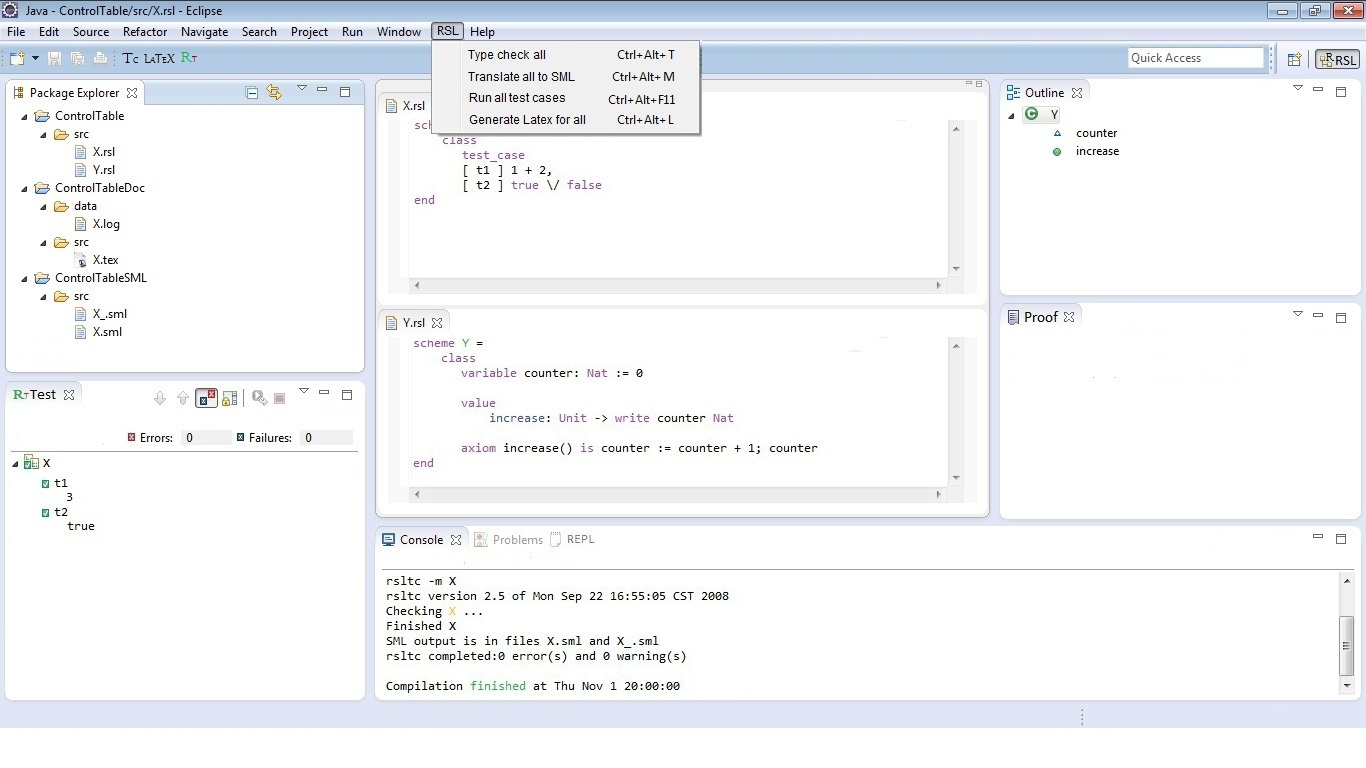
\includegraphics[width=2.5in]{RSLMenu.jpeg} 
% where an .eps filename suffix will be assumed under latex, 
% and a .pdf suffix will be assumed for pdflatex; or what has
% been declared via \DeclareGraphicsExtensions. 
%\caption{Eclipse user interface displaying the RSL menu item} 
%\label{UIMenu} 
%\end{figure}

\begin{figure*}[ht!] \centering
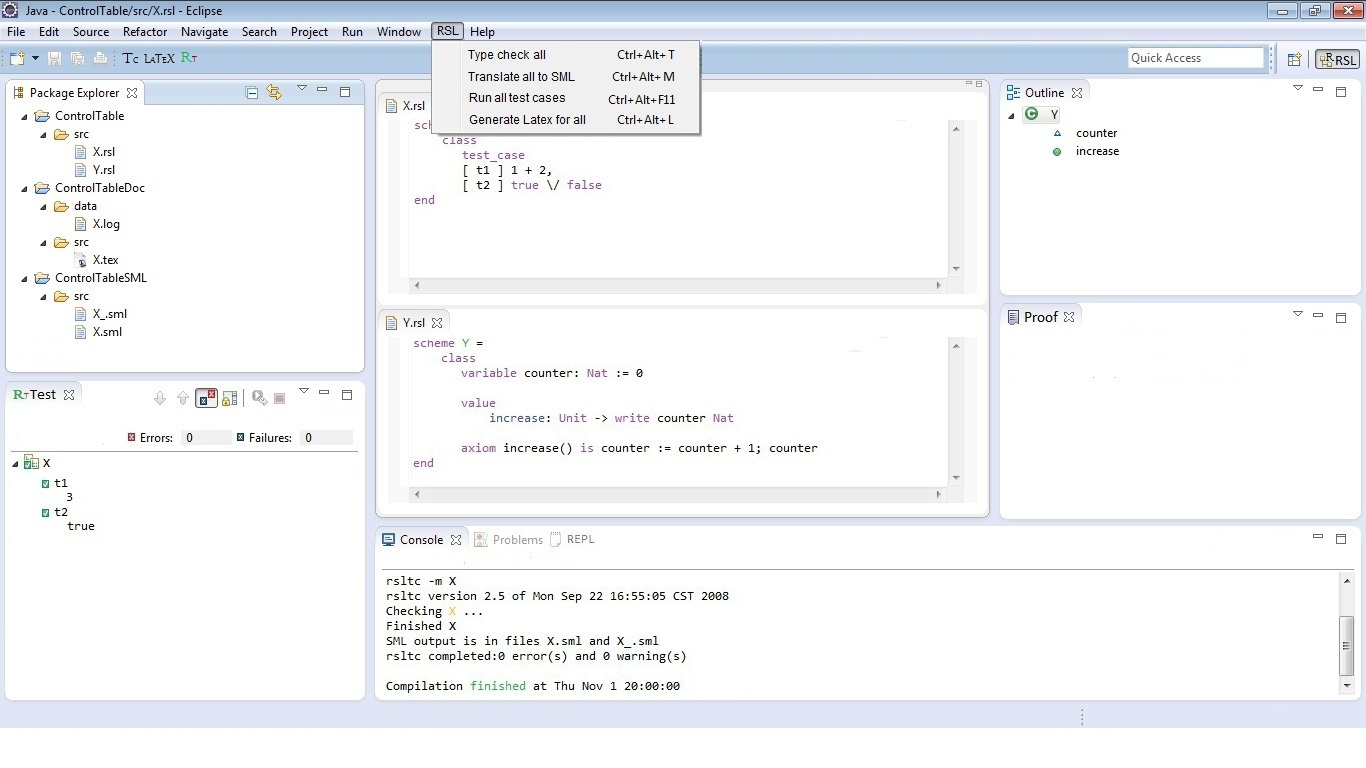
\includegraphics[width=7in]{RSLMenu.jpeg} 
% where an .eps filename suffix will be assumed under latex, 
% and a .pdf suffix will be assumed for pdflatex; or what has
% been declared via \DeclareGraphicsExtensions. 
\caption{Eclipse user interface displaying the RSL menu item} 
\label{UIMenu} 
\end{figure*}


\autoref{UIMenu} illustrates the graphical user interface for the
\emph{RSL} menu item.  This illustration was created by taking a
screenshot of Eclipse and then hand-editing the resulting image in
just a few minutes.

\lstset{style={bon}}
\lstinputlisting[style=bon, float=tp,label={example:scenario_chart},
caption={Scenario chart for RSL menu.},
captionpos=b]{scenario_example.bon}

While the user interface is being drawn, product requirements are
documented using EBON \emph{scenario\_chart} elements. The beautiful
part about using EBON is that it allows the requirements specification
to be captured using natural language. Therefore no intermediate step
is required between identifying the requirements and documenting them.
For the case study, the requirements associated with the user
interface in \autoref{UIMenu} are captured in the
\emph{scenario\_charts} in \autoref{example:scenario_chart}.

% Events
%
\subsection{Events}
\label{sec:events}

In this section the entire system is seen as a black box. The focus is
on the external actions that make the system react and on the system
outgoing responses. However, not all systems outgoing events are of
interest, but only the ones that are started by external stimuli. 

An incoming external event is any action that determines the system to
change its state. For example it can be a user clicking a button or
another system sending a request. An outgoing internal event is the
response the system sends to the one that initiated the incoming
external event. The system outgoing event for the action of pressing
the button could e.g. be the display of a new window or writing a
message to the standard output.

Looking back at the scenario presented in
\autoref{sec:user-interface}, the user has the possibility to type
check all RSL files. This is illustrated in \autoref{UIMenu} by the
presence of a sub-menu item named \emph{Type check all}. Therefore,
the incoming external action in this case is: \emph{the user selects
the Type check all sub-menu item}. And this external event has been
determined just by looking at the scenarios previously identified.
However, there is another user event that triggers the same system
reaction and that is using the shortcuts: \emph{The user presses
Ctrl+Alt+T}.

\lstset{style={bon}}
\lstinputlisting[style=bon, float=tp,label={example:event_chart_in},
caption={Incoming event chart for typechecking features.},
captionpos=b]{external_event_example.bon}

Once established, the user actions can be captured in EBON using
\emph{event\_chart} elements. The \emph{event\_chart} can be ingoing
or outgoing depending on the type of the events they capture. Since
the two user incoming events that have just been identified aims for
the same functionality, they are grouped under the same name
(\emph{TYPECHECKALL}) and captured in
\autoref{example:event_chart_in}. Please ignore for the moment the
\emph{involves} part in \autoref{example:event_chart_in}, since
\autoref{sec:comp-comm} will explain it in detail.

\lstset{style={bon}}
\lstinputlisting[style=bon, float=tp,label={example:event_chart_out},
caption={Outgoing event chart for typechecking features.},
captionpos=b]{internal_event_example.bon}


All incoming actions trigger changes in the system state. And the next
task is to decide how should the system notify the one triggering the
action, about the changes that have taken place. For the eRAISE case
study it was decided that after the user selects the \emph{Type check
all} sub-menu item, a message should be displayed on the standard
output. The message informs the user about how the typechecking
evolved and since the case study GUI is Eclipse based, the standard
output is considered by default the Eclipse Console view. However in
some cases the typechecking may not be successful due to some errors
in the input files. In this case it would be nice to know what caused
the problem and where can it be found. Therefore the system will
present the necessary information in the Eclipse Problem view. To sum
up, after the user selects the \emph{Type check all} sub-menu item,
the system updates the Console and Problem views with appropriate
information. \autoref{example:event_chart_out} presents the two events
captured in an outgoing \emph{event\_chart} under the names of
\emph{CONSOLEUPDATE}, respectively \emph{PROBLEMSUPDATE}.
\autoref{example:event_chart_out} also contains an \emph{involves}
part, which will be explained in detail in \autoref{sec:comp-comm}.


% Components
%
\subsection{Components}
\label{sec:components}

This subsection, in contrast with the previous one, looks inside the
system, at the components that form its architecture. These components
can be referring to concrete elements like a \emph{Zoom in button} or
they can be abstract concepts like \emph{User authentication} which
covers everything in the system responsible for authenticating a user.
Also multiple components can be grouped in a bigger component which
can also be part of another component.

The place to start identifying the system architecture components is
the domain model presented in \autoref{sec:domain-modeling}. The high
level classifiers captured there must be transformed into concrete
data types in order to bring the system development closer to the
implementation phase. The advantage of using EBON is that it
simplifies the transit between the domain model and architecture
and manages to capture the concrete data types in language
independent fashion. This is done by taking the entities captured in
\emph{system charts}, \emph{cluster charts} and \emph{class charts} and
transfer them in \emph{static diagrams}. An EBON \emph{static\_diagram}
contains multiple \emph{components} which can be \emph{clusters} or
\emph{classes} and which have the same meaning as the ones composing the
\emph{system\_chart} in \autoref{sec:domain-modeling}.

\lstset{style={bon}}
\lstinputlisting[style=bon, float=tp,label={example:system_architecture},
caption={System architecture caption},
captionpos=b]{system_architecture_example.bon}

Applying this step on the case study, the system chart presented in
\autoref{example:system_chart} becomes the SystemArchitecture from
\autoref{example:system_architecture}.
% Components communication
%
\subsection{Components communication}
\label{sec:comp-comm}

This section concern is how components interact with each other and
what interfaces they present to the other components that want to
communicate with them. The starting point is the list of incoming and
their corresponding outgoing actions identified in
\autoref{sec:events}. This helps identifying the components that react
first to an external stimuli and the components responsible for the
outgoing actions. Once the starting and ending point of the data flow
is established, the other interacting components are determined by
evaluating the scenarios in \autoref{sec:user-interface}. In EBON
notation, the components communication is seen in terms of
\emph{client, supplier} relationship. The component providing the
interface is a \emph{supplier} and all components using it are
\emph{clients}. In the eRAISE case study, one incoming event is
\emph{TYPECHECKALL} presented in \autoref{example:event_chart_in} and
its corespondent outgoing events are \emph{CONSOLEUPDATE} and
\emph{PROBLEMSUPDATE} presented in \autoref{example:event_chart_out}.
Thus the first component that reacts to user \emph{TYPECHECKALL}
action is the \emph{TypeChecker}. The component responsible for the
\emph{CONSOLEUPDATE} is the \emph{Console} and the one for
\emph{PROBLEMSUPDATE} is \emph{Problems}. The \emph{TypeChecker}
component typecheks the input and can directly inform the
\emph{Console} about the status. Therefore the \emph{TypeChecker} is a
client of \emph{Console} and this is expressed in EBON as: \emph{
TypeChecker client Console}. The client relations must be added in the
\emph{static\_diagram} after the components declaration.

%\note{Should I make a new BON example comprising client relations? -mvf}

Since \emph{TypeChecker} is directly stimulated by the
\emph{TYPECHECKALL} event and it is a client of \emph{Console} which
generates the outgoing response, it can be said that\emph{
TYPECHECKALL} event involves the \emph{TypeChecker} and the
\emph{Console} components. And this is how the \emph{involves} part in
\autoref{example:event_chart_in} is constructed. The same method is
applied to \emph{PROBLEMSUPDATE} event. This event is triggered if
there are errors displayed in the console. Therefore
\emph{TypeChecker} sends a message to \emph{Console} and if the
message is an error, a third component called \emph{ConsoleToProblems},
that monitors the \emph{Console}, notifies the \emph{Problems}
component. Therefor the \emph{PROBLEMSUPDATE} event involves the
\emph{TypeChecker, Console, ConsoleToProblems} and \emph{Problems}
components. This is captured in \autoref{example:event_chart_out}.


\lstset{style={bon}}
\lstinputlisting[style=bon, float=tp,label={example:interfaces},
caption={Console component interface},
captionpos=b]{interfaces_example.bon}


Once it was decided what components are interacting, it must be
established how do they accomplish that. This means establishing the
contracts between components by identifying the information a client
needs and the messages it sends to its supplier. EBON allows
specifying fully typed interfaces in an language independent mode
through the notion of \emph{feature}. Everything a component exposes
to its clients is called a feature. For example the \emph{Console}
component in the case study has a feature called \emph{update} which
allows the client components to sent it messages that will further be
displayed to the user. Please refer to the Console command in
\autoref{example:system_chart} for better understanding. These
messages are just strings and can be informative messages or errors.
The situation is captured in \autoref{example:interfaces}, where the
fully typed feature signature can be noticed. When a client calls
\emph{update} on the \emph{Console} it must send the message to be
displayed to the user and the information that specifies if it is an
error message or not. The assertion \emph{require} is a precondition
that makes sure that \emph{channel} is one of the values 1 or 2, where
1 stands for standard output and 2 for the standard error output. EBON
has also postcondition assertions named \emph{ensure}.

All these software contracts will later on, in the implementation phase,
result in plug-ins extensions and extension points.

% Code generation
%
\subsection{Code generation}
\label{sec:code-generation}

Once the analysis and design parts are finished, the next step is to
create the code skeleton. This part is done using a tool named Beetlz,
which automatically generates Java code from EBON
specification~\cite{Darulova09}.  The input of this tool is the EBON
\emph{system\_chart} and \emph{static\_diagram} that were obtained
throughout the entire analysis and design. With just one click, Beetlz
converts all EBON specification obtained in steps \emph{A} to \emph{E}
into Java elements.

% \note{-Joe, can you please add a bib item for the Beetlz tool? I used
% it the previous paragraph cite\{Beetlz\}. \\-And do we need a
% reference for Java?\\-And the code presented further down is not
% styled -mvf}

For example this is the Console class generated by Beetlz for the
component with the same name captured in \emph{static\_diagram} in
\autoref{example:interfaces}:

\begin{lstlisting}
public /*@ nullable_by_default @*/ class Console  {
   //@ ensures channel == 1 || channel == 2; public void
   update(List<Char> message, Channel channel){}
}
\end{lstlisting}

% =========================================================
% Conclusion
% =========================================================
\section{Conclusion}
\label{sec:conclusion}

The full specification of our case study is available in a technical
report version of this paper.  Its appendix contains all of the UI
sketches for the various plug-ins in the eRAISE feature, the high-level
concept/domain analysis, the specification of events, the architecture
specification, the formal component interface design, and the code
generated from that design.  The example plug-ins and feature are also
available in our repository at
GitHub.\footnote{\url{https://github.com/kiniry/eRAISE}}

The student responsible for the design and development of this plug-in
(the first author), had to learn and apply this methodology in only a
few short weeks.  That is evidence for its utility.  Only after
completing the plug-in will we be able to reflect upon how well the
analysis and design match the final implementation, but if past
projects using the EBON methodology are any indication, we expect to
see no architectural drift and full feature compliance.\footnote{Note
  to the reviewers: we expect that development will be complete by the
  time of the workshop so that we can demonstrate it in San Francisco.}

There are several opportunities for next steps refining this work in
the context of plug-in development.  

First, we would like to augment our advanced command-line options tool
suite ``CLOPS'' for plug-in development.  CLOPS permits one to
declaratively specific the syntax and semantics of the command-line
options of a tool.  CLOPS reasons about such specifications (it has a
formal semantics) and generates a lexer, parser, well-formedness
checker, and documentation.  Extending CLOPS to generate a set of
Eclipse plug-ins and architecture documentation, like that we
hand-write in this methodology, would be a valuable exercise and
product.

Second, the community should use this method to wrap several more
plug-ins following our example so that we can collectively properly
evaluate the methodology's utility.

% conference papers do not normally have an appendix

% use section* for acknowledgement
% \section*{Acknowledgment}
% \label{sec:acknowledgment}

% The authors would like to thank themselves by buying tons of chocolate
% and beer. They really deserve it. 

% trigger a \newpage just before the given reference
% number - used to balance the columns on the last page
% adjust value as needed - may need to be readjusted if
% the document is modified later
%\IEEEtriggeratref{8}
% The "triggered" command can be changed if desired:
%\IEEEtriggercmd{\enlargethispage{-5in}}

% references section

% can use a bibliography generated by BibTeX as a .bbl file
% BibTeX documentation can be easily obtained at:
% http://www.ctan.org/tex-archive/biblio/bibtex/contrib/doc/
% The IEEEtran BibTeX style support page is at:
% http://www.michaelshell.org/tex/ieeetran/bibtex/
%\bibliographystyle{IEEEtran}
% argument is your BibTeX string definitions and bibliography database(s)
%\bibliography{IEEEabrv,../bib/paper}
%
% <OR> manually copy in the resultant .bbl file
% set second argument of \begin to the number of references
% (used to reserve space for the reference number labels box)
%
\bibliographystyle{IEEEtran}
\bibliography{abbrev,main-bib}
%\begin{thebibliography}{1}

%\bibitem{IEEEhowto:kopka}
%H.~Kopka and P.~W. Daly, \emph{A Guide to \LaTeX}, 3rd~ed.\hskip 1em plus
% 0.5em minus 0.4em\relax Harlow, England: Addison-Wesley, 1999.

%\end{thebibliography}

% that's all folks
\end{document}
